\section{実験結果}
\subsection{粘度計測}
鋼球落下実験を行う試験溶液として,1wt.\%PAA溶液の製作を行った.この製作した溶液の粘度特性を確認し,先行研究\cite{ref:9}\cite{ref:10}における粘度特性と比較した.この比較を行うことで先行研究との粘度特性の違いを確認した.なお,この粘度計測を実施するためには,溶質が溶媒に十分に均一に溶解することならびに,混合時に混入した気泡がおおむね消失することが必要であるため,溶液製作1週間後に行った.それぞれの試料に対し,円錐回転子の回転数を変化させ,各5回計測を行いその平均を求めた.

水道水の粘度計測を行った結果をFig.\ref{fig:water-vis}に示す.なお,縦軸は粘度,横軸はせん断速度を表す.2.2においても示したが,コーンロータの回転速度を変化させることにより,せん断速度を変化させた.その結果,粘度は約1.1[Pa$\times$ s]でほぼ一定となっていた.これは,水がニュートン流体であり,粘度を比例係数とした速度勾配とせん断応力の比例関係となっているためであると考えられる.

水道水の場合と同様にPAA溶液の粘度計測を行った結果をFig.\ref{fig:PAA-vis}に示す.なお,縦軸は粘度の対数,横軸はせん断速度の対数を表す.また,Iwamuro {\it et al.}\cite{ref:9}やShiratori {\it et al.}\cite{ref:10}の文献値も共に示した.ここで,粘度$\mu$はせん断速度$\dot{\gamma}$に対して,粘度定数 k[Pa$\times$ $\text{s}^n$],指数$n$を用い Power-law modelに従うものとすると,
\begin{eqnarray}
    \label{eq:power-low}
    \mu=k\times\dot{\gamma}^{n-1}
\end{eqnarray}
といった式で与えられる\cite{ref:1}.式\ref{eq:power-low}を用いて近似線計算を行った結果,$k$=8.37[Pa$\times \text{s}^n]$,$n=0.24$であった.Iwamuro {\it et al.}\cite{ref:9}では,$k$=9.4[Pa$\times \text{s}^n]$,$n=0.23$と示されている.また,Shiratori {\it et al.}\cite{ref:10}を同様に解析すると,$k$=4.9[Pa$\times \text{s}^n$],$n=0.18$となっていた.今回作製したPAA溶液の粘度特性はIwamuro {\it et al.}とShiratori {\it et al.}の間に位置しており,適切に作製されたと判断できる.

\begin{figure}[ht]
    \centering
    \includegraphics[width=12cm,clip]{4-Results/water.png}
    \caption{Meansured viscosity versus shear rate for tap water.}
    \label{fig:water-vis}
\end{figure}

\begin{figure}[ht]
    \centering
    \includegraphics[width=13cm,clip]{4-Results/PAA-viscosity.png}
    \caption{Flow curve for 1wt.\%PAA solution.}
    \label{fig:PAA-vis}
\end{figure}

\newpage

\subsection{圧力場 計測結果}

容器Aにおける超音波圧力場の計測を行った結果をFig.\ref{fig:pressure}(a),容器Bにおける超音波圧力場の計測を行った結果をFig.\ref{fig:pressure}(b)に示す.縦軸は水槽底面からの高さ,横軸は圧力である.この結果を元にTable\ref{table:press-A},\ref{table:press-B} に圧力$P$の$y$方向平均値を示す.どちらの水槽においても水槽全体に圧力場が形成されていることが分かった.また,先行研究であるIwamuro \textit{et al}.\cite{ref:8},\cite{ref:9}と同様な圧力平均値となった.

\begin{table}[h]
    \centering
    \caption{Averaged value of pressure data in tank A.}
    \label{table:press-A}
    \begin{tabular}{c|c|c}\hline
                       & Present 1wt.\% PAA & Iwamuro {\it et al.}\cite{ref:8} \\ \hline
        $\bar{P}$[kPa] &       68        & 72                              \\ \hline
    \end{tabular}
\end{table}

\begin{table}[h]
    \centering
    \caption{Averaged value of pressure data in tank B.}
    \label{table:press-B}
    \begin{tabular}{c|c|c}\hline
                       & Present 1wt.\% PAA & Iwamuro \cite{ref:9} \\ \hline
        $\bar{P}$[kPa] & 159.2              & 180                              \\ \hline
    \end{tabular}
\end{table}

\begin{figure}[ht]
    \centering
    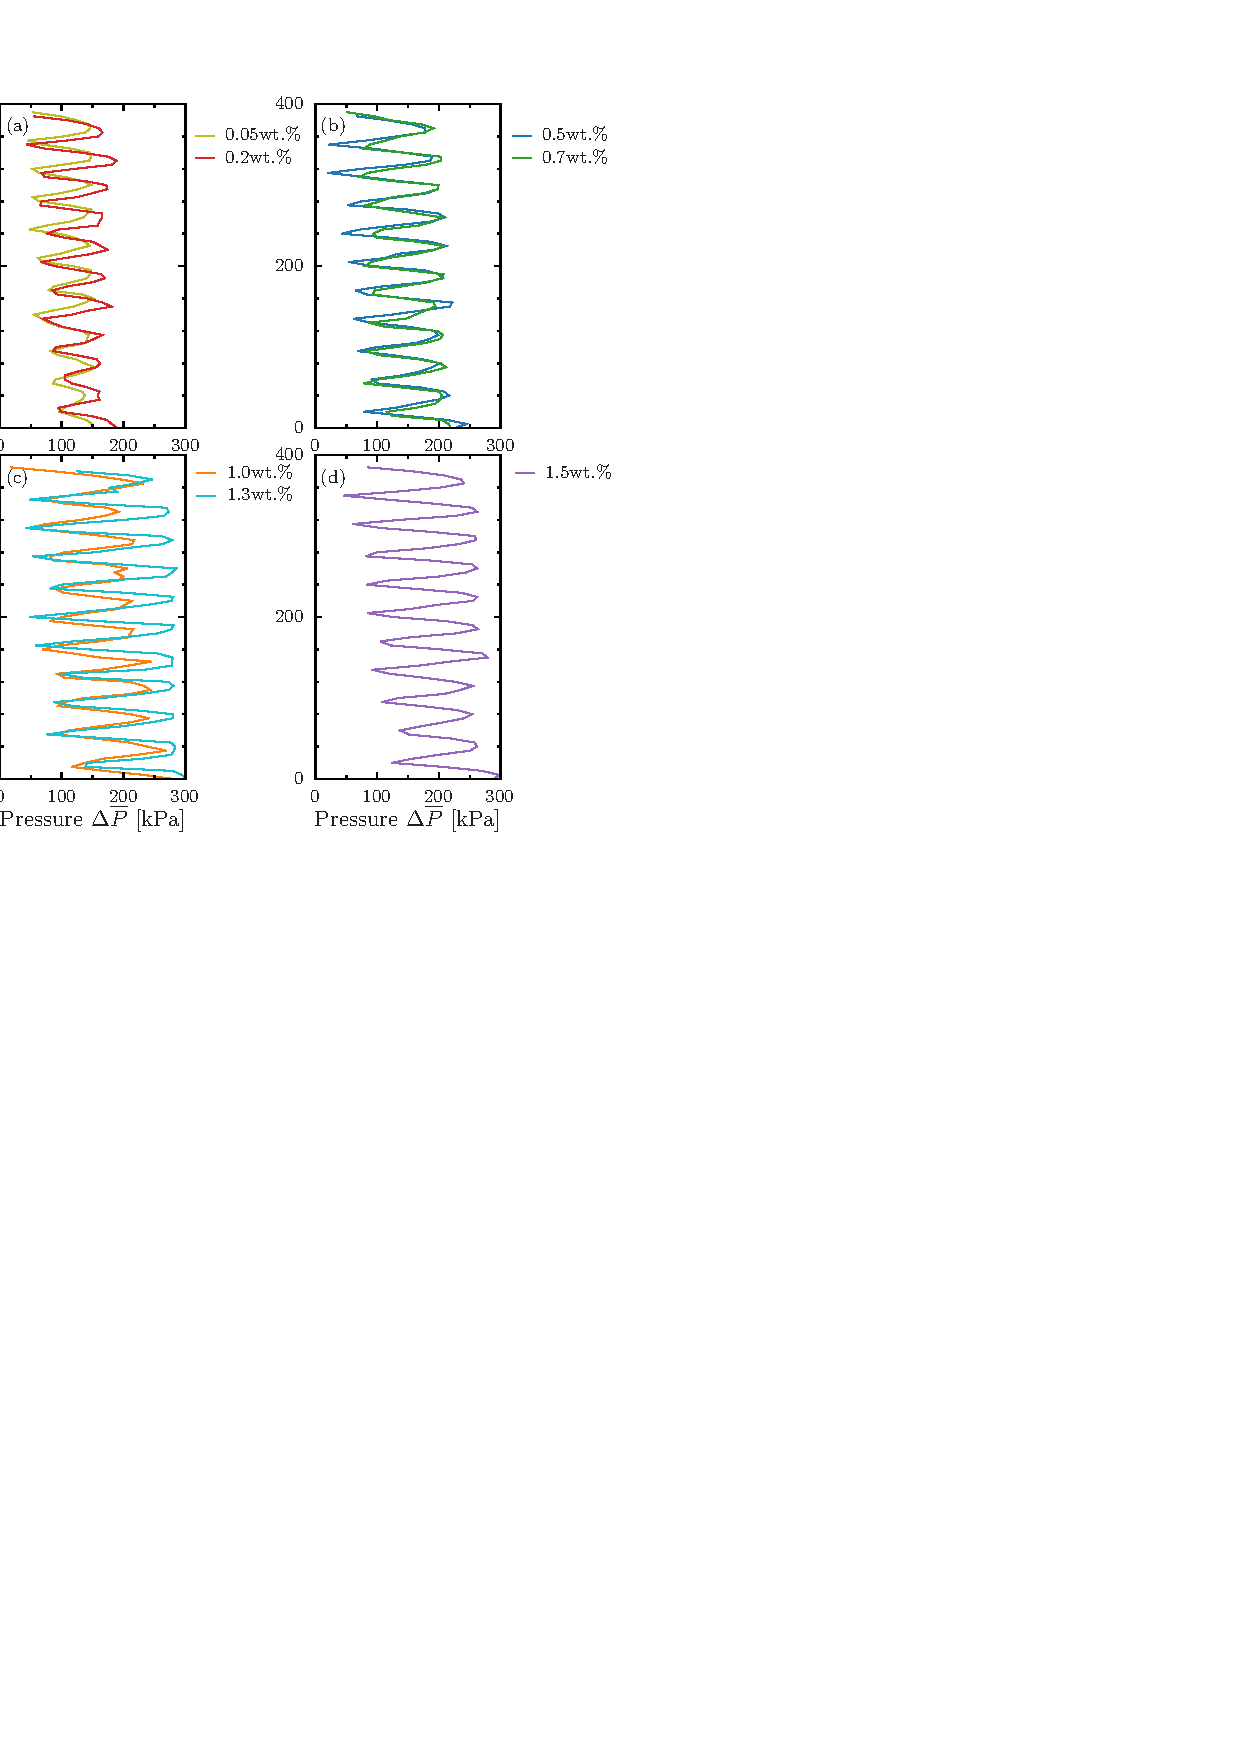
\includegraphics[width=12cm,clip]{4-Results/press.png}
    \caption{Pressure field in PAA solution measurement results. (a)In tank A. (b)In tank B.}
    \label{fig:pressure}
\end{figure}

\newpage

\subsection{装置改良における 実験結果}

容器Aにおいて真空ポンプを用いて球を把持し,球を落下させ解析した結果をFig\ref{fig:falling-A}に示す.縦軸は落下速度,横軸は落下開始時からの経過時間である.先行研究であるIwamuro \textit{et al}.\cite{ref:8}や電磁石を用いて球を把持した場合と比較し,超音波照射による高速化が顕著に現れていないことが分かる.


一方,今回行った真空ポンプを用いて把持した場合は,超音波照射の有無に関わらず,従来の手法における実験結果の間にあった.また,電磁石を用いた実験結果よりもよりIwamuro \textit{et al.}\cite{ref:8}の結果に近づいた.故に,実験手法として適切であることが分かった.なお,落下開始時に電磁石を用いた場合はオーバーシュートが見られるが,真空ポンプを用いた場合はオーバーシュートが見られなかった.これは実験手法の変化により弾性による影響が減少したためと考えられる.

\begin{figure}[ht]
    \centering
    \includegraphics[width=12cm,clip]{./4-Results/s1-A.png}
    \caption{Falling velocity of a sphere in 1wt.\%PAA solution with and without ultrasound irradiation in tank A.}
    \label{fig:falling-A}
\end{figure}

\newpage

\subsection{インターバル変化 実験結果}

容器Bにおいて落下間隔を5分,10分,20分と変化し,球を落下させた解析した結果をFig.\ref{fig:falling-5},\ref{fig:falling-10},\ref{fig:falling-20},に示す.縦軸は落下速度,横軸は落下開始時からの経過時間である.なお,落下間隔10分の結果に関して,比較のため先行研究であるIwamuro\cite{ref:9}における実験結果もあわせて示す.それぞれの場合において,超音波照射による落下球の高速化は見られた.

しかし,Iwamuro\cite{ref:9}と比較し,落下開始時の加速におけるオーバーシュートが今回は見られなかった.また,Iwamuro\cite{ref:9}においては落下速度は落下開始から0.8s以降,定常状態となっている.本実験において同条件である落下間隔10分において,超音波照射なしの場合,落下開始から0.2-0.7s間のみ,一定速度で落下し以降は加速した.オーバーシュートの有無は先述の装置改良における実験結果においても見られたため,実験手法の変化によるためだと考えられる.終端速度への到達の有無だが,擬塑性流体の粘弾性回復がIwamuro\cite{ref:9}と比較して十分に行われていないと考えられる.これは,落下間隔20分の条件において,Iwamuro\cite{ref:9}と同様の終端速度に達しているため,落下間隔10分では回復しきれなかった粘弾性が回復しきったためだと考えられる.粘弾性の回復時間が異なることに関しては,落下間隔をより細かく変化させ調査する必要があると考えられる.

\begin{figure}[ht]
    \centering
    \includegraphics[width=12cm,clip]{./4-Results/s1-5.png}
    \caption{Falling velocity of a sphere in 1wt.\%PAA solution with and without ultrasound irradiationin tank B. (Interval 5 min.)}
    \label{fig:falling-5}
\end{figure}
\begin{figure}[ht]
    \centering
    \includegraphics[width=12cm,clip]{./4-Results/s1-10.png}
    \caption{Falling velocity of a sphere in 1wt.\%PAA solution with and without ultrasound irradiationin tank B. (Interval 10 min.)}
    \label{fig:falling-10}
\end{figure}
\begin{figure}[ht]
    \centering
    \includegraphics[width=12cm,clip]{./4-Results/s1-20.png}
    \caption{Falling velocity of a sphere in 1wt.\%PAA solution with and without ultrasound irradiationin tank B. (Interval 20 min.)}
    \label{fig:falling-20}
\end{figure}

\clearpage
